\documentclass{scrartcl}
\usepackage[utf8]{inputenc}
\usepackage{listings}
\usepackage{graphicx}
\usepackage{cleveref}
\usepackage{hyperref}
\usepackage{floatrow}

\title{Dataset creation using Last.fm tags}
\subtitle{Audio and Music Processing Lab}
\author{Roman Tsukanov \\ SMC}
\date{March 15, 2016}

\begin{document}

\maketitle


\section{Introduction}

The goal of this lab was to use \href{https://last.fm/}{Last.fm} tags (other than genre) to create a dataset. Dataset then needs to be evaluated in AcousticBrainz project\footnote{\url{https://acousticbrainz.org/}}.

Last.fm tags come from a data dump, which contains tags mapped to MusicBrainz IDs (MBIDs)\footnote{\url{https://musicbrainz.org/doc/MusicBrainz\_Identifier}} of recordings. Each tag is associated with normalized count (0 being the least common tag and 100 the most common tag). Count indicates how many times users assigned a particular tag to a recording (track) on Last.fm. All recordings in that data dump have at least one low-level data submission on AcousticBrainz, so no filtering is required.

All scripts (Jupyter Notebooks\footnote{\url{https://jupyter.org/}}) and other materials are hosted at \url{https://github.com/gentlecat/amp-lab/tree/master/8_acousticbrainz}.


\section{Preparing and analyzing the data}

\textit{I used Python programming language for working with data and generating datasets.}

\subsection{Parsing}

Data dump was provided to us in CSV format\footnote{\url{https://tools.ietf.org/html/rfc4180}}. Each row contains MBID of a recording, followed by pairs of values: tag value, count for that tag.

To simplify further processing I created two Python dictionaries. First maps recording MBID to a list of \textit{\{tag, normalized count\}} tuples. Second maps tags to a list of \textit{\{recording MBID, normalized count\}} tuples.

\subsection{Looking at tags}

To see what tags are more popular I sorted them by number of occurrences. As a result I got a set of tags, which was used to define what kinds of datasets it is possible to create\footnote{I decided to create multiple datasets.}.

\begin{itemize}
    \item \textbf{Mood}: ["happy"], ["sad"]
    \item \textbf{Female/Male}: ["female vocalists", "female vocalist", "female vocals",
"female"], ["male vocalists", "male vocalist", "male vocals", "male"]
    \item \textbf{Quality of content}: ["good", "awesome", "amazing", "great"], ["bad",
"awful", "terrible", "garbage"]
    \item \textbf{Origin}: ["american", "usa"], ["british", "uk"], ["german", "deutsch",
"germany"], ["spanish", "spain"]
    \item \textbf{Rating (out of 10)}: ["0 of 10 stars"], ["1 of 10 stars"] ... ["10 of 10 stars"]
    \item \textbf{Decade}: ["20s"], ["30s"] ... ["90s"], ["2000s", "00s"], ["2010s", "10s"]
\end{itemize}

This list describes structure of datasets that I built. Each class can include recordings with one or more of specified labels. For example, it makes sense to combine recordings with tags ``male vocalists'' and ``male vocalist'', they mean pretty much the same thing in our context (Female/Male classification).


\section{Creating datasets for AcousticBrainz}

\subsection{Generating datasets from tags}

There are a couple of things to keep in mind when generating datasets:
\begin{enumerate}
    \item Classes need to have roughly the same number of items to prevent bias.
    \item There shouldn't be more than 1,000 instances in a class, because evaluation might take too much time.
\end{enumerate}

After looking at total number of instances I picked one that had lowest count or 1,000 (if it's more than that) and used it as a limit for all classes in a dataset.

Then I sorted all items in a class by normalized count. This was done to make sure that only items with higher count are used, assuming that they are better candidates for a particular class.

\subsection{Importing datasets into AcousticBrainz}

AcousticBrainz provides a way to import datasets in CSV format, so this is what I used to save them. Each row contains \textit{\{recording MBID, class name\}} pairs.

All datasets can be viewed on my AcousticBrainz profile page at \url{http://acousticbrainz.org/user/Gentlecat}. I submitted all of them for evaluation and already got some results.


\section{Results}

I got evaluation results for two datasets: ``Mood'' and ``Quality of content''. ``Mood'' classifier (Figure \ref{fig:mood}) has accuracy of $82.37\%$. ``Quality of content'' classifier (Figure \ref{fig:quality_of_content}) has accuracy of $71.11\%$. 

\begin{figure}[!h]
    \begin{floatrow}
        \ffigbox{
            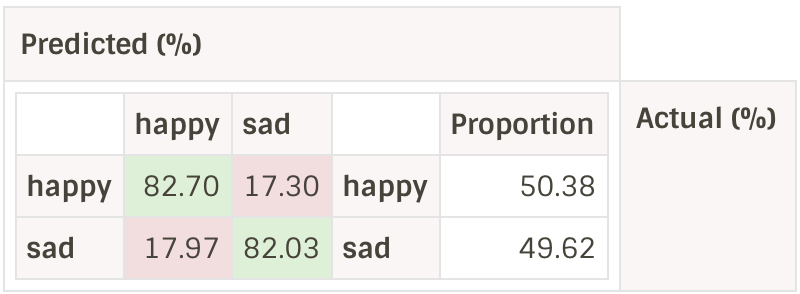
\includegraphics[width=0.4\textwidth]{mood.png}
        }{
            \caption{Confusion table for ``Mood'' classifier}
            \label{fig:mood}
        }
        \ffigbox{
            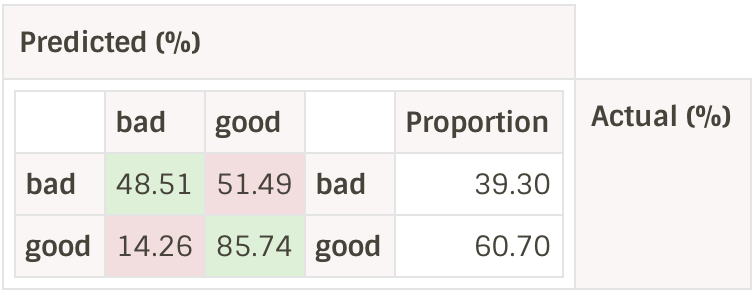
\includegraphics[width=0.4\textwidth]{quality_of_content.png}
        }{
            \caption{Confusion table for ``Quality of content'' classifier}
            \label{fig:quality_of_content}
        }
    \end{floatrow}
\end{figure}

Both results seem to be pretty good. It would be nice to check them against the rest of data that wasn't included into these datasets. Unfortunately, right now there's no easy way to do that.

Evaluation of other datasets has failed because of some issues in evaluation script.


\end{document}
